\begin{activity} \label{A:11.8.10}  We can use spherical coordinates to help us more easily understand some natural geometric objects.
    \ba
    \item Recall that the sphere of radius $a$ has spherical equation $\rho = a$.  Set up and evaluate an iterated integral in spherical coordinates to determine the volume of a sphere of radius $a$. 
    
    \item Set up, but do not evaluate, an iterated integral expression in spherical coordinates whose value is the mass of the solid obtained by removing the cone $\phi=\frac{\pi}{4}$ from the sphere $\rho = 2$ if the density $\delta$ at the point $(x,y,z)$ is $\delta(x,y,z) = \sqrt{x^2+y^2+z^2}$.  An illustration of the solid is shown in Figure \ref{F:11.8.Spherical_ex2}.
\begin{figure}[ht]
\begin{center}
%\resizebox{!}{2.75in}{\includegraphics{11_8_Spherical_ex2}}
  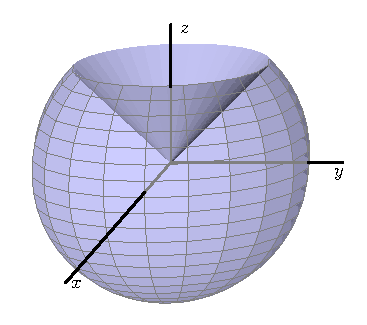
\includegraphics{figures/fig_11_8_sphere_cone.eps}
\end{center}
\caption{The solid cut from the sphere $\rho = 2$ by the cone $\phi=\frac{\pi}{4}$.}
\label{F:11.8.Spherical_ex2}
\end{figure}
    \ea



\end{activity}
\begin{smallhint}

\end{smallhint}
\begin{bighint}

\end{bighint}
\begin{activitySolution}

\ba
\item Recall that the volume of a solid $S$ is given by
\[\int \int \int_S \, dV.\]
Thus, the volume of a sphere of radius $a$ can be calculated as an iterated integral as follows:
\begin{align*}
\int \int \int_S \, dV &= \int_0^{2\pi} \int_0^{\pi} \int_0^{a} \rho^2 \sin(\phi) \, d\rho \, d\phi \, d\theta \\
	&= \int_0^{2\pi} \int_0^{\pi} \left. \left[\frac{\rho^3}{3} \sin(\phi) \right]\right|_0^a  \, d\phi \, d\theta \\
	&= \int_0^{2\pi} \int_0^{\pi} \frac{a^3}{3} \sin(\phi) \, d\phi \, d\theta \\
	&= \int_0^{2\pi} \left. \left[-\frac{a^3}{3} \cos(\phi)\right]\right|_0^{\pi} \, d\theta \\
	&= \int_0^{2\pi} 2\frac{a^3}{3} \, d\theta \\
	&= \frac{4}{3}\pi a^3.
\end{align*}


\item The limits on $\rho$ are $0 \leq \rho \leq 2$ and on $\theta$ are $0 \leq \theta \leq 2\pi$. To account for the cone being removed from the sphere we restrict $\phi$. The cone opens from $\phi = 0$ to $\phi = \frac{\pi}{4}$, so the limits on $\phi$ that remove the cone are $\frac{\pi}{4} \leq \phi \leq \pi$. Therefore, the density of the solid is found by 
\[\int_{0}^{2\pi} \int_{\pi/4}^{\pi} \int_0^2 \rho^3 \sin(\phi) \, d\rho \, d\phi \, d\theta.\]
\ea

\end{activitySolution}
\aftera
